% !TeX root = ../tfg.tex
% !TeX encoding = utf8

\chapter{Análisis empírico del Deep Double Descent}\label{ch:analisis-empirico-ddd}

\section{Materiales y métodos}\label{sec:materiales-y-metodos}

\subsection{Datasets}\label{subsec:datasets}

En la parte práctica de este proyecto, se emplearán diversos conjuntos de datos (datasets) etiquetados, pues nos movemos bajo el enfoque del aprendizaje supervisado. Dado que la experimentación se limita a este tipo de aprendizaje, se han seleccionado datasets ampliamente reconocidos y utilizados en problemas de clasificación de imágenes, lo que también nos ayudará a comparar los resultados obtenidos con los de la comunidad científica. A continuación, se detallarán los principales datasets utilizados en este estudio: MNIST, CIFAR-$10$, CIFAR-$100$, Flowers$102$.\newline


Cabe destacar que, aunque en este proyecto también se utilizan datasets sintéticos, estos no serán mencionados en esta sección, pues se detallarán en el propio experimento, y la descripción se centrará exclusivamente en los conjuntos de datos comentados anteriormente.\newline

\subsubsection{MNIST}\label{subsubsec:MNIST}

El dataset MNIST (Modified National Institute of Standards and Technology)~\cite{LeCun2005TheMD} es un conjunto de datos de imágenes ampliamente utilizado para tareas de clasificación. Consta de $70000$ imágenes en escala de grises de dígitos escritos a mano, las cuales se dividen en $60000$ imágenes para entrenamiento y $10000$ para test. Además, cada imagen tiene un tamaño de $28 \times 28$ píxeles.\newline

\subsubsection{CIFAR-10 y CIFAR-100}\label{subsubsec:CIFAR10-y-CIFAR100}

CIFAR-$10$~\cite{Krizhevsky2009} es un conjunto de datos utilizado para tareas de clasificación. Consta de $60000$ imágenes en color, distribuidas en 10 clases diferentes, cada una con $6000$ imágenes. A su vez, estas imágenes se dividen en $50000$ imágenes para entrenamiento y $10000$ para test. Cada imagen tiene un tamaño de $32 \times 32$ píxeles y está en formato RGB, es decir, cada imagen cuenta con $3$ capas, cada una asociada con un color del formato RGB.\newline

Por otro lado, CIFAR-$100$~\cite{Krizhevsky2009} es un conjunto de datos similar a CIFAR-$10$, pero con $100$ clases. Consta de $60000$ imágenes en color, divididas en $100$ clases de $600$ imágenes cada una, con $500$ para entrenamiento y $100$ para test. Las imágenes tienen un tamaño de $32 \times 32$ píxeles en formato RGB.\newline

\subsubsection{Flowers102}\label{subsubsec:Flowers102}

El dataset Flowers$102$~\cite{Nilsback2008} es un conjunto de datos utilizado comúnmente en tareas de clasificación de imágenes, especialmente en el reconocimiento de imágenes de flores. Este dataset contiene $102$ categorías diferentes de flores, con un total de $8189$ imágenes de resolución variable en formato RGB, aunque la mayoría tienen un tamaño de $224 \times 224$ píxeles. Cada categoría de flores incluye entre $40$ y $258$ imágenes, lo que permite que el dataset tenga diversidad de muestras dentro de cada clase.\newline

La distribución de las imágenes dentro del dataset es la siguiente: $1020$ imágenes se utilizan para entrenamiento, $1020$ imágenes para validación y $6149$ imágenes para el conjunto de test. La gran diferencia en el número de imágenes entre los conjuntos de entrenamiento/validación y el conjunto de test hace que este dataset sea particularmente complicado de predecir, dado que las condiciones de las imágenes (ángulos, fondos y luces) varían considerablemente entre las clases.\newline

Para asegurar que todas las imágenes de este dataset tengan las mismas dimensiones y reducir la complejidad computacional, las imágenes se escalan a una resolución de $32 \times 32$ píxeles en formato RGB. Al reducir la resolución de las imágenes, se facilita el entrenamiento de los modelos, aunque se podría comprometer significativamente su capacidad para aprender características relevantes para la clasificación.\newline

Para terminar esta sección, se presenta una tabla a modo de resumen de los datasets que se utilizarán en este proyecto. La Tabla~\ref{tab:datasets} muestra la información relevante sobre cada uno de los datasets, incluyendo el número total de imágenes, el tamaño de las imágenes y el número de características (píxeles totales), lo que proporciona una visión general de sus características principales y facilita la comparación entre ellos.\newline

\begin{table}[h]
    \centering
    \begin{tabular}{|c|c|c|c|c|}
    \hline
    \textbf{Dataset} & \textbf{Nº imágenes} & \textbf{Tamaño imagen} & \textbf{Clases} & \textbf{Entrada} \\
    \hline
    MNIST & $70000$ & $28 \times 28$ píxeles (escala de grises) & $10$ & $784$ \\
    CIFAR-$10$ & $60000$ & $32 \times 32$ píxeles (RGB) & $10$ & $3072$ \\
    CIFAR-$100$ & $60000$ & $32 \times 32$ píxeles (RGB) & $100$ & $3072$ \\
    Flowers$102$ & $8189$ & $32 \times 32$ píxeles (RGB) & $102$ & $3072$ \\
    \hline
    \end{tabular}
    \caption[Resumen de los datasets utilizados.]{Resumen de los datasets utilizados. En la tabla aparecen las principales características de cada dataset, donde la última columna hace referencia al número total de píxeles de cada imagen.}\label{tab:datasets}
\end{table}

Aunque los datasets elegidos no son excesivamente grandes, con el fin de acelerar el proceso de entrenamiento durante un alto número de épocas, se utilizarán subconjuntos de estos datasets en los experimentos. En particular, cuando se haga uso de un subconjunto, se empleará la siguiente notación:

\[
    \text{dataset}[\text{train/test}]
\]

donde $\text{dataset}$ se refiere a uno de los conjuntos de datos previamente definidos, $\text{train}$ indica el número de ejemplos utilizados para entrenamiento, y $\text{test}$ representa el número de ejemplos en el conjunto de prueba. Un ejemplo sería MNIST($4000/1000$), donde se indica que estamos utilizando un subconjunto de MNIST con 4000 ejemplos de entrenamiento y 1000 para test.\newline

\subsection{Arquitecturas utilizadas}\label{subsec:arquitecturas}

En esta sección se presentan las arquitecturas diseñadas y utilizadas con el objetivo de abordar la tarea de clasificación propuesta por los datasets comentados en la sección anterior. Las arquitecturas seleccionadas varían en términos de su complejidad (número de parámetros) y del tipo de capas que incorporan, desde modelos simples hasta configuraciones más profundas.\newline

Este enfoque permitirá analizar el impacto del \textit{Deep Double Descent} en los distintos casos que puede presentarse y sobre las distintas arquitecturas. A continuación, se describen en detalle las arquitecturas implementadas, justificando su elección y su relevancia en el contexto de este estudio.\newline

\subsubsection{2NN}\label{subsubsec:2NN}

Como primer modelo se propone una arquitectura muy simple, formada únicamente por dos capas densas. Para ello, primeramente se añade una capa de aplanamiento \textit{(flattening)} con el objetivo de convertir las imágenes proporcionadas en la entrada en un vector de píxeles unidimensional. A continuación, se añade la primera capa densa, cuya entrada está compuesta por el vector unidimensional anterior y su salida será un número variable de neuronas, todas ellas conectadas con cada entrada del vector. Finalmente, la última capa densa conectará las neuronas de salida de la primera capa densa con un número de neuronas que será igual al número de clases del datasets con el que estemos trabajando.\newline

El diseño y elección de este modelo se basa en su relativa sencillez, que será de gran utilidad a la hora de realizar diversidad de experimentos, lo que lo convierte en una opción ideal para llevar a cabo una amplia variedad de experimentos al permitir tiempos de entrenamiento significativamente más bajos en comparación con otras arquitecturas utilizadas.\newline

Finalmente, se expone una tabla con el número de parámetros que conforman esta arquitectura. Este detalle es especialmente relevante para los experimentos, ya que el número de parámetros reflejará el nivel de complejidad de la arquitectura (véase Tabla~\ref{tab:numero-parametros}).\newline

\begin{table}[ht]
    \centering
    \renewcommand{\arraystretch}{1.5} 
    \begin{tabular}{|c|c|c|}
    \hline
    \textbf{Arquitectura}          & \textbf{Entrada}                                   & \textbf{Número de parámetros}                     \\ \hline
    $2$NN                & Imagen de tamaño $n \times n \times l$                & $(n^2 \times l) \times k + k + c \times k + c$                                             \\ \hline
    \end{tabular}
    \caption[Resumen de las arquitecturas $2$NN.]{Resumen de las arquitecturas $2$NN. En la tabla se muestra el número de parámetros dada una determinada imagen de entrada, donde $k$ hace referencia al número de neuronas de salida de la primera capa densa y $c$ al número de clases del problema de clasificación.}\label{tab:numero-parametros}
\end{table}

\subsubsection{ResNet-18 modificada}\label{subsubsec:resnet18-modificada}

ResNet-$18$ es una de las variantes de la famosa arquitectura de redes neuronales convolucionales ResNet (Residual Networks), propuesta por Kaiming He y su equipo en 2015~\cite{He2015}. Esta arquitectura fue diseñada con el objetivo de resolver el problema de la degradación del rendimiento a medida que aumentaba la profundidad de las redes neuronales. Para solucionarlo, ResNet introduce el concepto de las conexiones residuales, que permiten que el flujo de información pase a través de capas sin ser afectado por los gradientes de las capas anteriores.\newline

ResNet-$18$, como su nombre indica, tiene $18$ capas de profundidad. Su arquitectura presenta varios bloques de convolución seguidos de conexiones residuales, que permiten que la entrada de cada bloque se sume a la salida de dicho bloque. La primera capa convolucional utiliza un filtro de tamaño $7 \times 7$ y, acto seguido, aparecen los bloques convolucionales formados por $4$ capas convolucionales idénticas, donde cada bloque está formado por dos capas convolucionales con conexiones residuales conectadas con la salida de la segunda capa convolucional. Finalmente, aparece una capa densa que será la salida de la red (véase Figura~\ref{fig:resnet18} para más detalle).\newline

\begin{figure}[h]
    \centering
    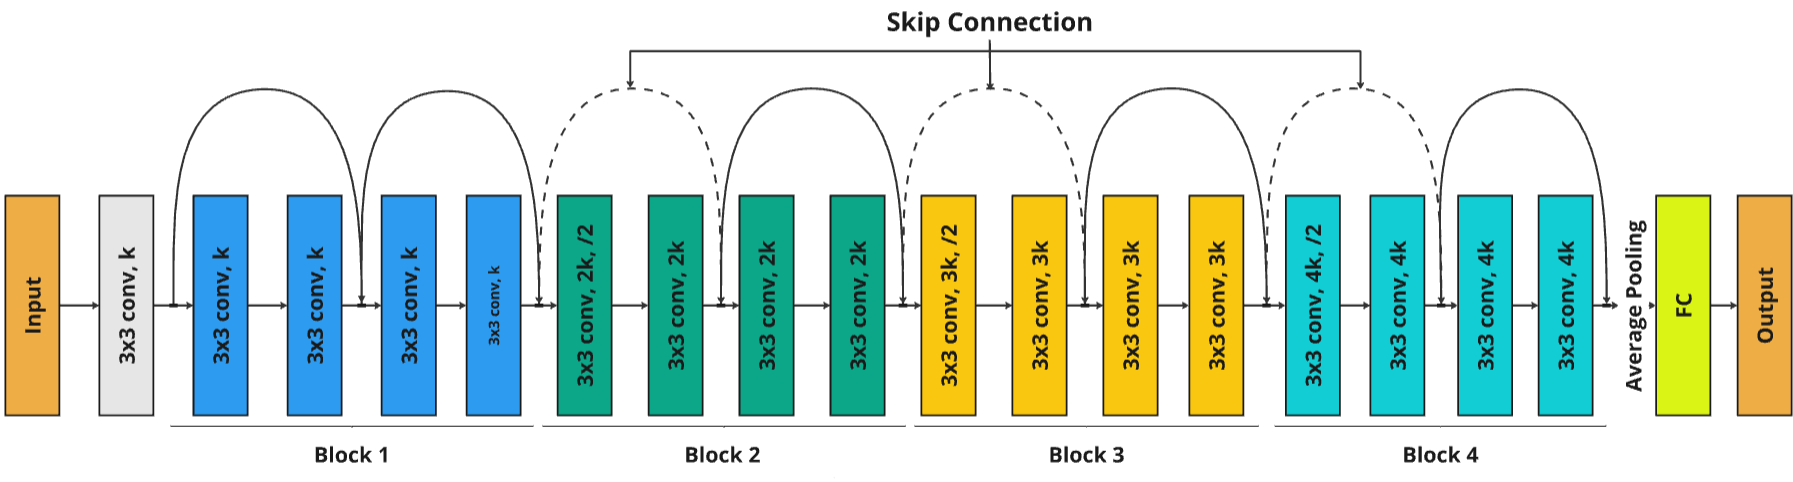
\includegraphics[width=\linewidth]{img/experiments/resnet18modified.png}
    \caption[Arquitectura ResNet$18$ modificada.]{Arquitectura ResNet$18$ modificada. Podemos observar los 4 bloques convolucionales (distinguidos por color), cada uno de ellos con su correspondiente número de filtros ([$k$, $2k$, $3k$, $4k$] con $k \in \mathbb{N}$), junto con las conexiones residuales. Imagen original del autor.}\label{fig:resnet18}
\end{figure}

La arquitectura que usaremos durante el transcurso de los experimentos es una modificación de la arquitectura ResNet$18$ original, dado que, en la arquitectura original el número de filtros usados en cada bloque convolucional es [$64$, $128$, $256$, $512$], mientras que en nuestro caso será un número variable $k \in \mathbb{N}$, con el propósito de poder modificar el número de parámetros de la red y crear ``distintas'' arquitecturas.\newline

Para ello, usaremos como número de filtros para cada bloque convolucional la secuencia: [$k$, $2k$, $3k$, $4k$]~\cite{Nakkiran2019}, con el objetivo de comparar los resultados obtenidos con los de la literatura existente. Destacamos que, para el valor $k=64$, nuestra arquitectura es la propia arquitectura ResNet-$18$ original.\newline

Finalmente y dado que el número de parámetros asociados a esta arquitectura es tedioso de indicar (debido a la gran cantidad de capas que la conforman), se expone una tabla con los principales valores del parámetro $k$ (número de filtros) utilizados en el desarrollo de la práctica (véase Tabla~\ref{tab:numero-parametrosresnet}).\newline

\begin{table}[ht]
    \centering
    \begin{tabular}{|c|c|c|}
    \hline
    \textbf{Valor de $k$}           & \textbf{Número de parámetros}                     
    \\ \hline
    $20$                  & $\approx 1.1$\space M                                            \\ \hline
    $45$                  & $\approx 5.5$\space M                                             \\ \hline
    $64$                  & $\approx 11.1$\space M                                             \\ \hline
    \end{tabular}
    \caption[Número de parámetros de las arquitecturas ResNet$18$ modificadas.]{Número de parámetros de las arquitecturas ResNet$18$ modificadas. Se muestra el número de parámetros dada un determinado valor $k$ y para $10$ clases de salida.}\label{tab:numero-parametrosresnet}
\end{table}

\subsubsection{3CNN}\label{subsubsec:3CNN}

Siguiendo la misma idea de la subsección anterior, en la que se varía el número de filtros en cada capa convolucional, se propone una nueva arquitectura compuesta por $3$ capas convolucionales (denominada $3$CNN), seguidas de capas de \textit{pooling} para reducir dimensionalidad y, finalmente, una capa densa de salida.\newline

Este modelo se presenta como una opción intermedia en términos de complejidad entre los dos modelos expuestos previamente, donde el número de filtros en cada capa se ajustará según un parámetro $k \in \mathbb{N}$, siguiendo la secuencia [$k$, $2k$, $4k$] (véase Figura~\ref{fig:3CNN}).\newline

\begin{figure}[h]
    \centering
    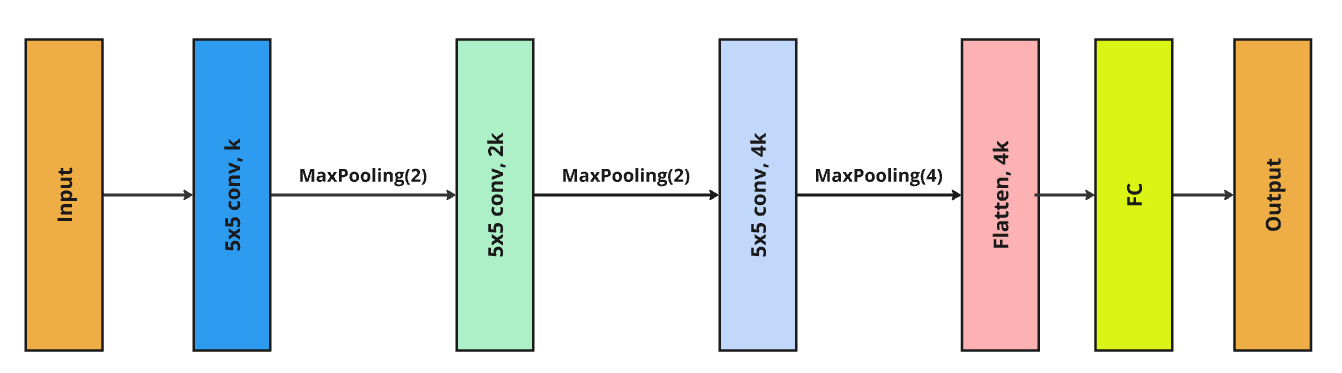
\includegraphics[width=\linewidth]{img/experiments/3CNN.png}
    \caption[Arquitectura $3$CNN.]{Arquitectura $3$CNN. Podemos observar los 3 bloques convolucionales (distinguidos por color), cada uno de ellos con su correspondiente número de filtros ([$k$, $2k$, $4k$] con $k \in \mathbb{N}$). Imagen original del autor.}\label{fig:3CNN}
\end{figure}

Finalmente, la Tabla~\ref{tab:numero-parametros3cnn} muestra el número de parámetros para algunos valores del parámetro $k$, lo que permite realizar una comparación con la arquitectura ResNet anterior.

\begin{table}[ht]
    \centering
    \begin{tabular}{|c|c|c|}
    \hline
    \textbf{Valor de $k$}           & \textbf{Número de parámetros}                     
    \\ \hline
    $20$                  & $\approx 103$\space K                                            \\ \hline
    $45$                  & $\approx 512$\space K                                             \\ \hline
    $64$                  & $\approx 1,03$\space M                                             \\ \hline
    \end{tabular}
    \caption[Número de parámetros de las arquitecturas $3$CNN.]{Número de parámetros de las $3$CNN. Se muestra el número de parámetros dada un determinado valor $k$ y para $10$ clases de salida.}\label{tab:numero-parametros3cnn}
\end{table}

\subsection{Hiperparámetros}\label{subsec:hiperparametros}

Los hiperparámetros que serán utilizados a lo largo de la experimentación, por lo general, son los valores por defecto que vienen con las implementaciones estándar de Pytorch~\cite{NEURIPS2019_9015} de los distintos métodos utilizados. Las únicas modificaciones que se han realizado son aquellas necesarias para replicar experimentos descritos en la literatura existente y, en dichos casos, se indicarán específicamente en el propio experimento.\newline

En cuanto al tamaño del lote (\textit{batch size}), variará entre $128$ y $256$, de manera similar a la literatura existente, lo que representa un valor relativamente alto, con el objetivo de acelerar el proceso de entrenamiento. Respecto a la tasa de aprendizaje del optimizador utilizado (Adam en nuestro caso), se empleará la tasa por defecto. El uso de distintos valores para \textit{batch size} y \textit{learning rate} en un problema donde se manifiesta el doble descenso se pueden observar en el Apéndice~\ref{ap:apendiceC}, donde se muestra que, si el fenómeno ocurre, el tamaño del lote utilizado y la tasa de aprendizaje no afectan significativamente al comportamiento del mismo.\newline

Por otra parte, cabe destacar que, salvo que se indique lo contrario, no se introduce ninguna técnica de regularización en los experimentos realizados, debido a que el \textit{Deep Double Descent} se observará sin la influencia de las mismas. De este modo, se pretende estudiar cómo se manifiesta este suceso bajo condiciones más puras, sin modificaciones que podrían alterar sus efectos. Cualquier variación en este aspecto será especificada de manera explícita en el propio experimento. Adicionalmente, como función de pérdida a minimizar se utilizará la entropía cruzada, dado que estamos trabajando con problemas de clasificación multiclase.\newline

\section{Experimentos}\label{sec:experimentos}

En esta sección se presentará una batería de resultados obtenidos a partir de los experimentos realizados, los cuales incluyen tanto resultados favorables como desfavorables, con el propósito de proporcionar una visión lo más completa posible de los mismos.\newline

\subsection{Aproximación polinómica de Legendre}\label{subsec:approx-legendre1}

Este primer experimento sirve como preámbulo al resto de experimentos y tiene como objetivo proporcionar una comprensión clara y sencilla de por qué puede manifestarse el \textit{Deep Double Descent} al aumentar la complejidad de un modelo. A través de este análisis preliminar, se busca sentar las bases para explorar más a fondo cómo la complejidad afecta al comportamiento y rendimiento de los modelos en los experimentos posteriores.\newline

Para ello, se busca replicar el resultado de la Imagen $2$ de~\cite{Schaeffer2023} (véase Figura~\ref{fig:1DDD}). El experimento trata de aproximar una función objetivo ($y(x) = 2x + \cos(25x)$) mediante el uso de la aproximación polinómica de Legendre para distintos grados de dicho polinomio y sobre un conjunto de $10$ puntos obtenidos al muestrear la función anterior. Este experimento no utilizará redes neuronales, sino que se basa en una simple regresión polinómica.\newline

\begin{figure}[h]
    \centering
    \begin{minipage}{0.32\textwidth}
        \centering
        \textbf{Región infraparametrizada} \\[0.5ex] 
        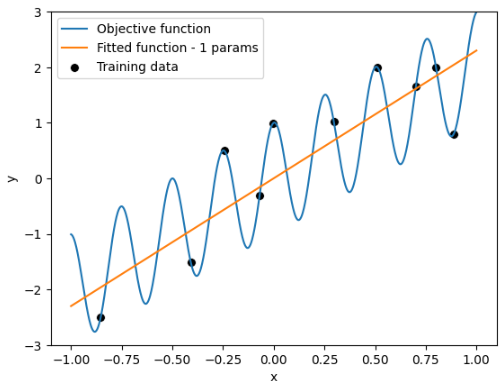
\includegraphics[width=\linewidth]{img/experiments/legendre1.png}
    \end{minipage}
    \begin{minipage}{0.32\textwidth}
        \centering
        \textbf{Umbral de interpolación} \\[0.5ex] 
        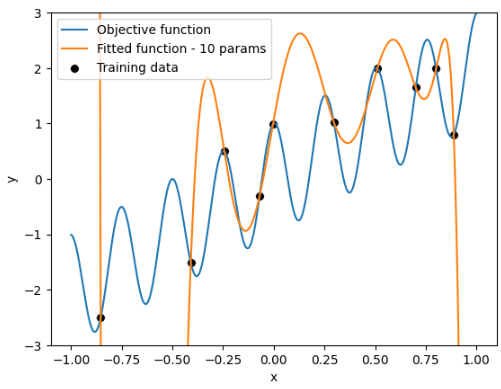
\includegraphics[width=\linewidth]{img/experiments/legendre2.png}
    \end{minipage}
    \begin{minipage}{0.32\textwidth}
        \centering
        \textbf{Región sobreparametrizada} \\[0.5ex] 
        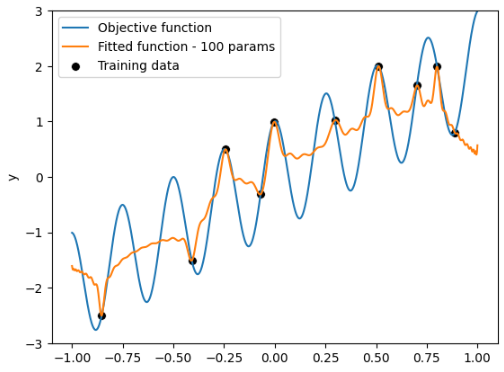
\includegraphics[width=\linewidth]{img/experiments/legendre3.png}
    \end{minipage}
    \caption[Intuición del \textit{Deep Double Descent} usando regresión polinómica.]{Intuición del \textit{Deep Double Descent} usando regresión polinómica. Cuando nos encontramos en la región infraparametrizada, el modelo no es capaz de capturar todos los datos de entrenamiento, haciendo que el bias del modelo sea grande, aunque la varianza sea pequeña. En el umbral de interpolación, el modelo captura perfectamente todos los datos, haciendo que el bias sea pequeño pero la varianza sea grande, pues la función aprendida dependerá de la posición de los datos de entrenamiento. Finalmente, en la región sobreparametrizada, el modelo está ``regularizado'' hacia una solución de norma pequeña.}\label{fig:1dd}
\end{figure}

Al alcanzar el umbral de interpolación, el modelo se ve obligado a ajustarse exactamente a cada uno de los puntos de entrenamiento, lo que lo convierte en una solución única. En este caso, el grado del polinomio coincide con el número de puntos, lo que no asegura garantizar una buena generalización debido a la ``rigidez'' del modelo al presentar numerosos ``picos'' (véase Figura~\ref{fig:1dd}).\newline

Al superar dicho umbral, el modelo adquiere mayor flexibilidad para aproximar los datos, lo que da lugar a una función cada vez más ``suave''. Además, el aumento en el número de parámetros más allá de dicho umbral permite la existencia de múltiples modelos de interpolación para cada grado, facilitando la selección de una opción que generalice bien. Esto puede observarse en la Figura~\ref{fig:1DDD}.\newline

\begin{figure}[h]
    \centering
    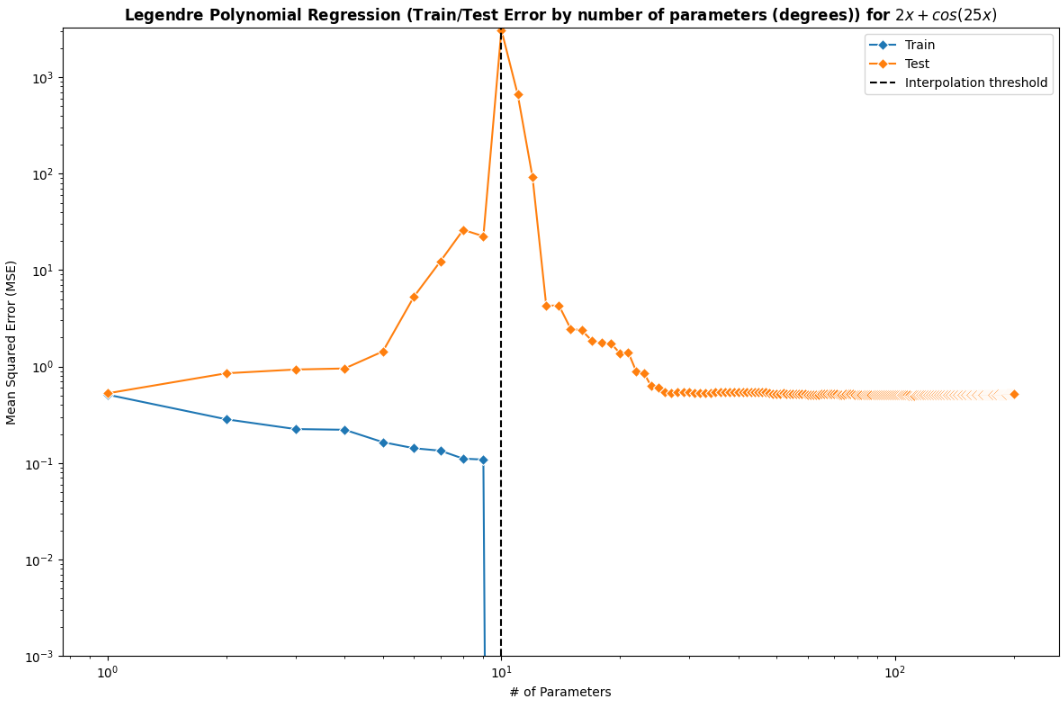
\includegraphics[width=0.5\textwidth]{img/experiments/legendreDDD.png}
    \caption[Doble descenso al utilizar aproximación polinómica de Legendre.]{Doble descenso al utilizar aproximación polinómica de Legendre, donde el umbral de interpolación corresponde al número de datos de entrenamiento.}
    \label{fig:1DDD}
\end{figure}

\subsubsection{Función cuadrática}\label{subsubsec:cuadratica}

\subsubsection{Función exponencial}\label{subsubsec:exponencial}

\subsubsection{Función hiperbólica}\label{subsubsec:hiperbolica}

\subsection{Noise-wise double descent}\label{subsec:noise-wise-dd}

En esta subsección, y como preámbulo al resto de experimentos, se estudia cómo varía el doble descenso al aumentar el porcentaje de ruido en las etiquetas. De este modo, añadimos este tipo de doble descenso a las variantes clásicas propuestas por Nakkiran et al.\ en~\cite{Nakkiran2019}.\newline

Para ello, se llevará a cabo un experimento con la arquitectura $2$NN sobre el dataset MNIST[$4000/1000$], modificando el porcentaje de ruido añadido en las etiquetas y entrenando cada modelo durante $1000$ épocas.\newline

\begin{figure}[h]
    \centering
    \begin{minipage}{0.45\textwidth}
        \centering
        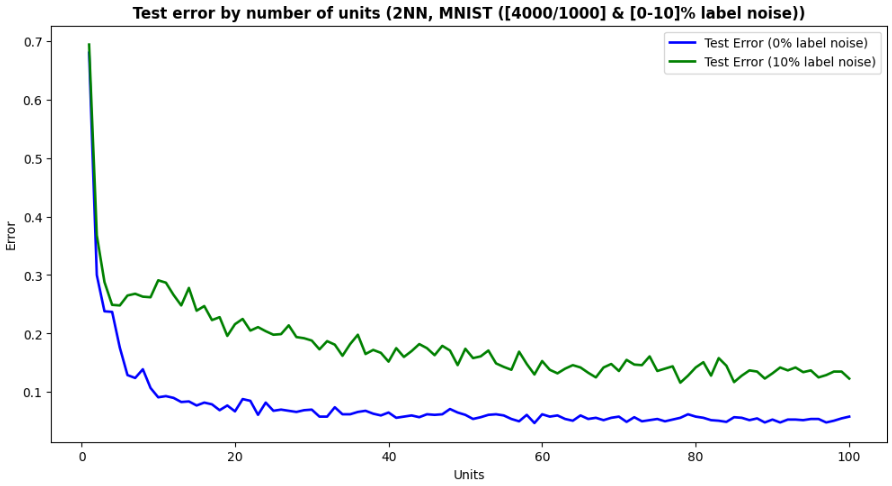
\includegraphics[width=\linewidth]{img/experiments/noise-wise-dd1.png}
    \end{minipage}
    \begin{minipage}{0.45\textwidth}
        \centering
        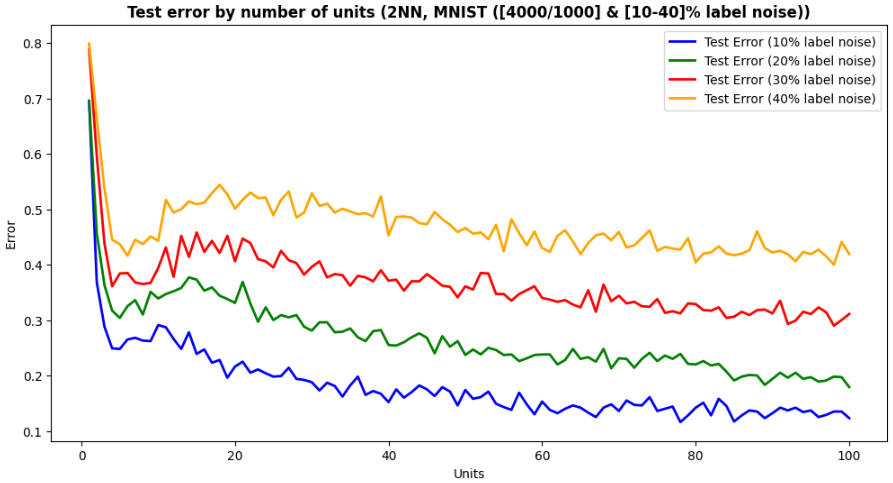
\includegraphics[width=\linewidth]{img/experiments/noise-wise-dd2.png}
    \end{minipage}
    \caption[Doble descenso para distintos niveles de ruido.]{Error en test de la arquitectura 2NN sobre el subconjunto MNIST[$4000/1000$] para diferente nivel de ruido. A la izquierda, en ausencia de ruido añadido, el doble descenso no se manifiesta. En cambio, a la derecha, al aumentar el nivel de ruido, el pico de la curva se vuelve cada vez más pronunciado.}\label{fig:noise-wise-dd}
\end{figure}

En la Figura~\ref{fig:noise-wise-dd} se observa que un modelo que no presenta doble descenso sobre el conjunto de datos original sí lo experimenta al agregarle ruido. Además, en modelos donde si aparece el doble descenso, el pico del error de test aumenta al incrementar el porcentaje de ruido, ya que el modelo, eventualmente, memorizará dicho ruido, lo cual concuerda con lo planteado en la literatura científica.\newline

También se aprecia que, a medida que aumenta el ruido, se requieren más parámetros para alcanzar errores de test más bajos que el mínimo obtenido durante el primer descenso. Este fenómeno, junto con el aumento del tiempo de entrenamiento al incrementar el ruido (véase Tabla~\ref{tab:noisewisedd}) y considerando que, en escenarios reales, el porcentaje de ruido no suele ser excesivamente alto, nos lleva a optar por configuraciones con un nivel de ruido en torno al $10-20\%$ para los experimentos restantes.\newline

Finalmente, en la Figura~\ref{fig:noise-wise-dd3} podemos verificar cómo, al aumentar el porcentaje de ruido en las etiquetas, el umbral de interpolación se desplaza hacia la derecha.\newline

\begin{figure}[h]
    \centering
    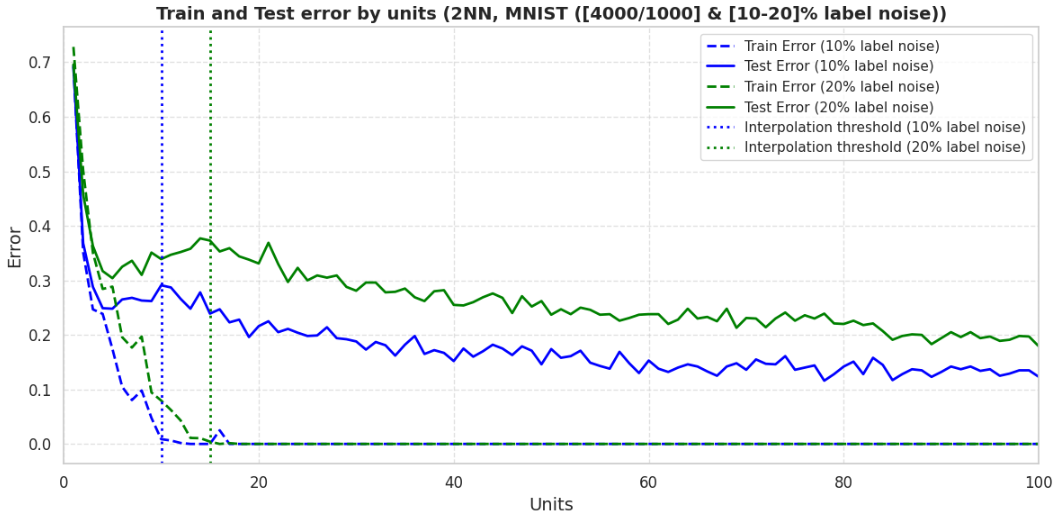
\includegraphics[width=0.5\textwidth]{img/experiments/noise-wise-dd3.png}
    \caption[Umbral de interpolación para el doble descenso con distintos niveles de ruido.]{Error en entrenamiento, test y umbral de interpolación respecto a la arquitectura $2$NN sobre el subconjunto MNIST[$4000/1000$] con distinto nivel de ruido añadido en las etiquetas.}\label{fig:noise-wise-dd3}
\end{figure}

\begin{table}[h!]
    \centering
    \begin{tabular}{|c|c|c|c|}
    \hline
    \textbf{Modelo}       & \textbf{Dataset} & \textbf{Ruido en etiquetas} & \textbf{Entrenamiento} \\ 
    \hline
    $2$-NN ($1-100$)          & MNIST[$4000/1000$]        & $\times$         & $26$h $10$min       \\ 
    $2$-NN ($1-100$)          & MNIST[$4000/1000$]        & $10\%$         & $26$h $50$min       \\ 
    $2$-NN ($1-100$)          & MNIST[$4000/1000$]        & $20\%$         & $27$h $23$min       \\ 
    $2$-NN ($1-100$)          & MNIST[$4000/1000$]        & $30\%$          & $28$h $8$min       \\ 
    $2$-NN ($1-100$)          & MNIST[$4000/1000$]       & $40\%$          & $30$h $14$min       \\  
    \hline
    \end{tabular}
    \caption[Resumen de los experimentos para el doble descenso por nivel de ruido.]{Resumen de los experimentos para el doble descenso por nivel de ruido.}
    \label{tab:noisewisedd}
    \end{table}

\subsection{Sample-wise double descent}\label{subsec:sample-wise-dd}

En esta subsección se presentan los experimentos realizados para analizar el \textit{sample-wise double descent}, el cual se manifiesta al modificar la cantidad de datos empleados durante el entrenamiento de un modelo específico. Este comportamiento destaca una zona de interés donde, al comparar las curvas del error de prueba, se observa que entrenar con un mayor número de ejemplos puede, de manera casi paradójica (en el sentido que, generalmente, en el aprendizaje automático siempre se busca tener la mayor cantidad de datos posible de cara a entrenar), empeorar el rendimiento del modelo.\newline

Dado que la experimentación presentada en la literatura existente resulta excesivamente costosa de replicar, se han diseñado experimentos más accesibles que permiten analizarlo manteniendo un enfoque lo suficientemente representativo.\newline

La idea para crear estos experimentos sencillos surge del hecho de que si un determinado modelo presenta \textit{model-wise doble descent} para un determinado número de ejemplos de entrenamiento, si aumentamos el número de ejemplos de entrenamiento, el pico del error de test se desplazará hacia la derecha (véase la imagen izquierda de la Figura~\ref{fig:swdd}), creando una región, que denominamos zona de interés.\newline

Dentro de esta zona se verifica que entrenar con más ejemplos puede empeorar el rendimiento del modelo (véase la zona sombreada en color rojo de la Figura~\ref{fig:swdd}). Sin embargo, es importante resaltar que, fuera de esta zona específica, el entrenamiento con un mayor número de ejemplos suele ser beneficioso para el rendimiento general del modelo, es decir, el modelo debería obtener menor error de test (el área bajo la curva de error fuera de dicha región debe ser menor para el modelo entrenado con un mayor número de ejemplos).\newline

Por tanto, para la realización de este experimento se utilizará la red $2$NN, donde el número de unidades de salida de la primera capa densa variará desde $1$ hasta $200$ y entrenaremos cada modelo durante $1000$ épocas. Además, se utilizará el dataset MNIST, sobre el que se extraeran $4000$ y $8000$ ejemplos para los distintos experimentos a realizar y a los que se les agregará un ruido del $10$\% en sus etiquetas.\newline

\begin{figure}[h!]
    \centering
    \begin{minipage}{0.49\textwidth}
        \centering
        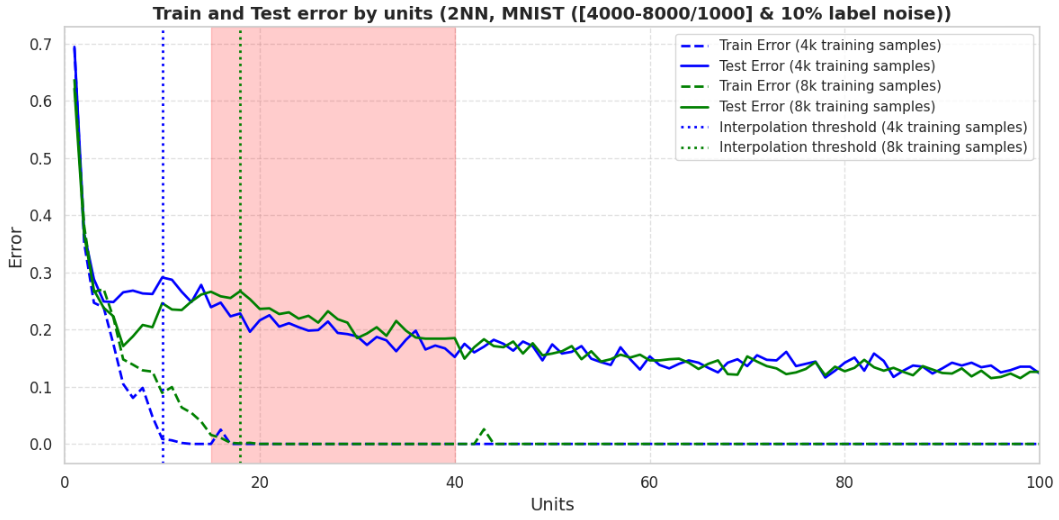
\includegraphics[width=\linewidth]{img/experiments/sample-wise-dd1.png}
    \end{minipage}
    \hfill
    \begin{minipage}{0.49\textwidth}
        \centering
        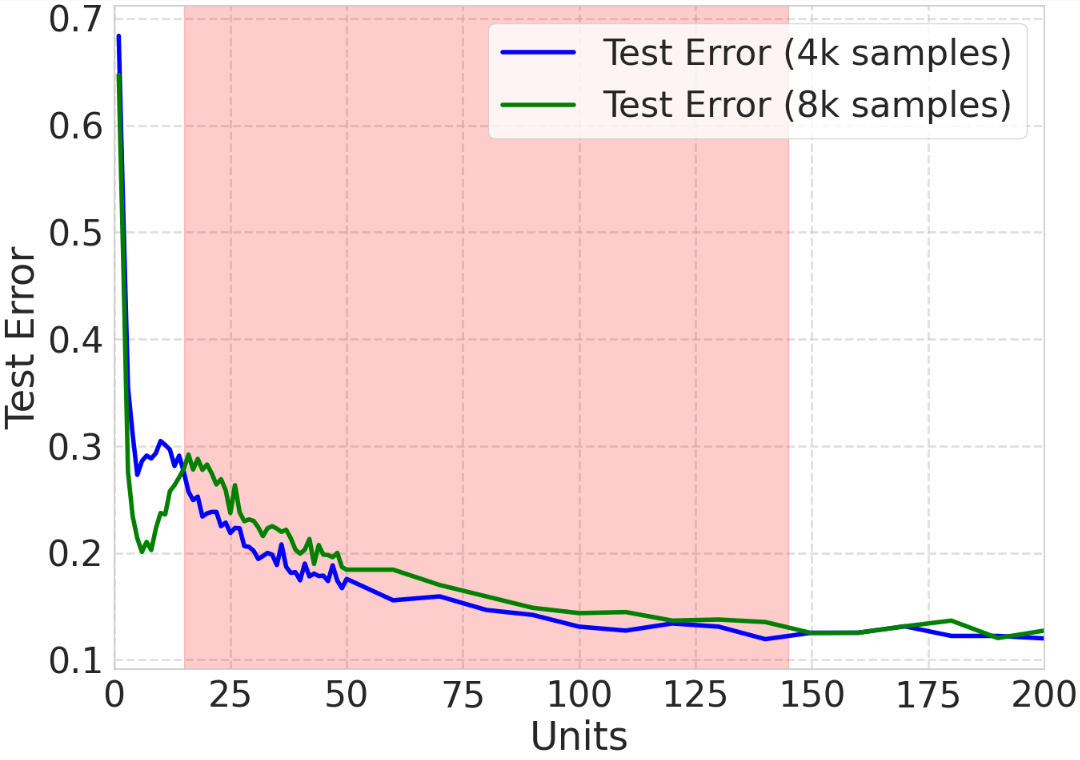
\includegraphics[width=\linewidth]{img/experiments/sample-wise-dd2.png}
    \end{minipage}
    \caption[Ejemplo de \textit{sample-wise double descent}.]{Ejemplo de \textit{sample-wise double descent} para la red $2$NN sobre dos subconjuntos de MNIST, utilizando $4000$ y $8000$ ejemplos de entrenamiento. A la izquierda aparece el resultado de una única realización del experimento. A la derecha aparece el resultado obtenido al realizar la media de $3$ experimentos.}
    \label{fig:swdd}
\end{figure}

Al igual que ocurría al aumentar el nivel de ruido, si aumentamos el número de ejemplos de entrenamiento, el umbral de interpolación también se desplaza hacia la derecha (véase la imagen izquierda de la Figura~\ref{fig:swdd}). Es decir, el modelo requiere de un mayor número de parámetros para memorizar un mayor número de ejemplos de entrenamiento, lo que, a priori, parece tener sentido con la complejidad efectiva del modelo.\newline

Finalmente, se muestra en la Tabla~\ref{tab:model_training_time} el tiempo de ejecución necesario para la realización de este experimento. Cabe destacar que, en el experimento donde se calcula la media de $3$ ejecuciones, se utiliza el modelo $2$NN hasta $50$ unidades (de $1$ en $1$) y, a partir de este valor, se suman las unidades de $10$ en $10$ hasta llegar a $200$ unidades, con el propósito de acelerar el entrenamiento fuera de la zona de interés que proporcionaba el primer experimento.\newline

\begin{table}[h!]
\centering
\begin{tabular}{|c|c|c|}
\hline
\textbf{Modelo}       & \textbf{Dataset} & \textbf{Entrenamiento} \\ 
\hline
$2$-NN ($1-100$)      & MNIST[$4000/1000$]         & $26$h $50$min       \\ 
$2$-NN ($1-100$)      & MNIST[$8000/1000$]         & $59$h       \\ 
$2$-NN ($1-200$) $\times$ $3$     & MNIST[$4000/1000$]         & $53$h $10$min       \\ 
$2$-NN ($1-200$) $\times$ $3$      & MNIST[$8000/1000$]         & $104$h $30$min       \\ 
\hline
\end{tabular}
\caption[Resumen de los experimentos para el doble descenso por número de ejemplos de entrenamiento.]{Resumen de los experimentos para el doble descenso por número de ejemplos de entrenamiento.}
\label{tab:model_training_time}
\end{table}

\section{Conclusión}\label{sec:conclusion-informatica}

\endinput